
% \iffalse
\let\negmedspace\undefined
\let\negthickspace\undefined
\documentclass[journal,12pt,twocolumn]{IEEEtran}
\usepackage{cite}
\usepackage{amsmath,amssymb,amsfonts,amsthm}
\usepackage{algorithmic}
\usepackage{graphicx}
\usepackage{textcomp}
\usepackage{xcolor}
\usepackage{txfonts}
\usepackage{listings}
\usepackage{enumitem}
\usepackage{mathtools}
\usepackage{gensymb}
\usepackage{comment}
\usepackage[breaklinks=true]{hyperref}
\usepackage{tkz-euclide} 
\usepackage{listings}
\usepackage{gvv}                                        
\def\inputGnumericTable{}                                
\usepackage[latin1]{inputenc}                            
\usepackage{color}                                       
\usepackage{array}                                       
\usepackage{longtable}                                   
\usepackage{calc}                                        
\usepackage{multirow}                                    
\usepackage{hhline}                                      
\usepackage{ifthen}                                      
\usepackage{lscape}
\usepackage{amsmath}
\newtheorem{theorem}{Theorem}[section]
\newtheorem{problem}{Problem}
\newtheorem{proposition}{Proposition}[section]
\newtheorem{lemma}{Lemma}[section]
\newtheorem{corollary}[theorem]{Corollary}
\newtheorem{example}{Example}[section]
\newtheorem{definition}[problem]{Definition}
\newcommand{\BEQA}{\begin{eqnarray}}
\newcommand{\EEQA}{\end{eqnarray}}
\newcommand{\define}{\stackrel{\triangle}{=}}
\theoremstyle{remark}
\newtheorem{rem}{Remark}



\usepackage{amsmath} % Include the amsmath package for align environment

\begin{document}

\bibliographystyle{IEEEtran}

\vspace{3cm}

\title{NCERT Physics Chapter-15 Q7}
\author{EE23BTECH11059 - Tejas$^{}$}
\maketitle

\newpage

\Huge \textbf{QUESTION 7:} \\

\medskip
\Large
A hospital uses an ultrasonic scanner to locate tumors in a tissue. What is the
wavelength of sound in the tissue in which the speed of sound is $1.7 \, \text{km/s}$? The operating frequency of the scanner is $4.2 \, \text{MHz}$.
\bigskip
\\
\Large
\textbf{SOLUTION:} \\

\\
Using the relation between wavelength($\lambda$), frequency($f$) and speed of sound in a medium($v$)\\
\begin{align}
    c&=f\lambda \\
     \lambda&=c/f
\end{align}
\begin{table}[h]
    \centering  
    \begin{tabular}{|c|c|c|}
        \hline
        Input Parameter & Value & Description  \\
        \hline
        $c$ & $1.7\times10^3$ m/s & Speed of Wave   \\
        \hline
        $f$ & $4.2\times10^6$ Hz & Frequency   \\
        \hline
        $A$ & 1 & Wave Amplitude  \\
        \hline
        
        
    \end{tabular}
\end{table}
The general equation of a sound wave is
\begin{align}
y\brak{t}=A \sin (2\pi\text{f} t-kx)
\end{align}
\begin{table}[h]
    \centering
    \begin{tabular}{|c|c|c|c|}
        \hline
        Input Paramter & Value & Description & Formulae  \\
        \hline
        A& 1&Amplitude& - \\
        \hline
        $f$& $4.2\times10^6$& Frequency& - \\
        \hline
        $k$& $4.04\times10^-4$ & Wave Number & $\frac{2\pi}{\lambda}$ \\
        \hline
        $x$ & Arbitrary & Position & - \\
        \hline
    \end{tabular}
    \
\end{table}

\\ 

\vspace{3cm}
\begin{figure}[h]
    \centering
    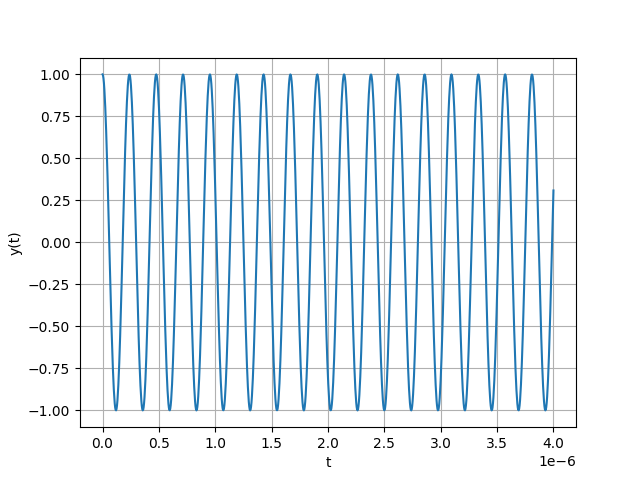
\includegraphics[width=\columnwidth]{images/plot.png}
    \caption{Waveplot}
    \label{fig:Plot1}
\end{figure} 
The frequency of sound relates to the pitch of that
sound, the higher the frequency, the higher the pitch
and lower the frequency lower the pitch. For
example, the voice frequency of males and females
are different in their adulthood (Generally females have a higher frequency of voice than
males) and the frequency of small kids is even
more than that.



The Amplitude of sound refers to the loudness of
sound i.e. intensity of the sound. The higher the
amplitude higher the loudness and the lower the
amplitude, the lower the loudness. The SI unit amplitude is meter (m)

K is called as the wave number, it gives an idea
about how many waves are present in a unit
length (here it is a meter), So the higher the wave
length lower the wave number and lower the
wavelength higher the wave number.

Physically, the wavelength of a sound wave
can be visualized as the distance between
two successive compressions (high-pressure regions) or rarefactions (low-pressure regions)
in the air or any other medium through which
the sound is propagating.
\section*{\Large Physical interpretation of speed of sound}
The speed of a sound wave in a medium can be interpreted in a physical manner without directly referencing its frequency and wavelength. The speed of sound is determined by the properties of the medium through which it travels, primarily its density (
$\rho$) and elasticity.\\

The general formula for the speed of sound in a medium is given by:
$$\text{v}=\sqrt{ \frac{\gamma \cdot P}{\rho}}$$
where:
\begin{itemize}
    \item v is the speed of sound
    \item $\gamma$ is the adiabatic index or ratio of specific heats
    \item $P$ is the pressure of the medium
    \item $\rho$ is the density of the medium.
\end{itemize}







        
        
        
             
             
        

        













\renewcommand{\thefigure}{\theenumi}
\renewcommand{\thetable}{\theenumi}





\end{document}
